\section{Proposed Method}
In this section, we design a framework for time and context aware session-based news recommendation to solve the challenges that news recommender meets. 

First, considering that each session is anonymous and short, which means the whole task is based on user-cold-start scenario, we formulate the session-based news recommendation task as a sequential prediction task, making it suitable for this data streaming setting. When new users starts a session and clicks several articles, we aim to recommend personalized articles based on their behavior within the session. Second, instead of denoting each item as an one-hot high-dimensional vector followed by an embedding layer, we train topic-oriented embedding vector for each article based on it's textual content to alleviate item-cold-start problem. Third, aiming to learn fluctuations of user intra-session behavior, we deploy multi-head attention transformer to obtain the representation of present reading motivations. After this, the recommendation task is reduced to a classification between the target article and negative candidates, which are sampled from k-nearest neighbors according to inter-session similarity.

There are two key factors revealed to model complex time-varying patterns: (1) \textbf{intra-session} temporal information: each user interaction within a session is companied with two types temporal value $T_j$, the \textit{publish} time of article that the user clicks $Tp_j$ and the \textit{click} time $Tc_j$ (reflecting the position of this interaction in the session). The sequence of $T_j$ represents the temporal information within the session, thus we encode it as time decay weighting for corresponding user interaction representation. (2) \textbf{inter-session} temporal information: each session begins at different time $T_u$, and temporally closer sessions tend to have more relations. Then we can generate candidates from top-K most similar sessions using the time-aware similarity measure.

In Section~\ref{sec:3.1} we introduce the embedding extracting of the article content. Then we introduce how to leverage multi-head self attention mechanism on excavating sequential and intra-session temporal information of user interactions in Section~\ref{sec:3.2}. Next, in Section~\ref{sec:3.3} we introduce different negative sampling strategies, and how to make use of inter-session temporal information in negative sampling.

\begin{figure*}[!htp]
    \centering
    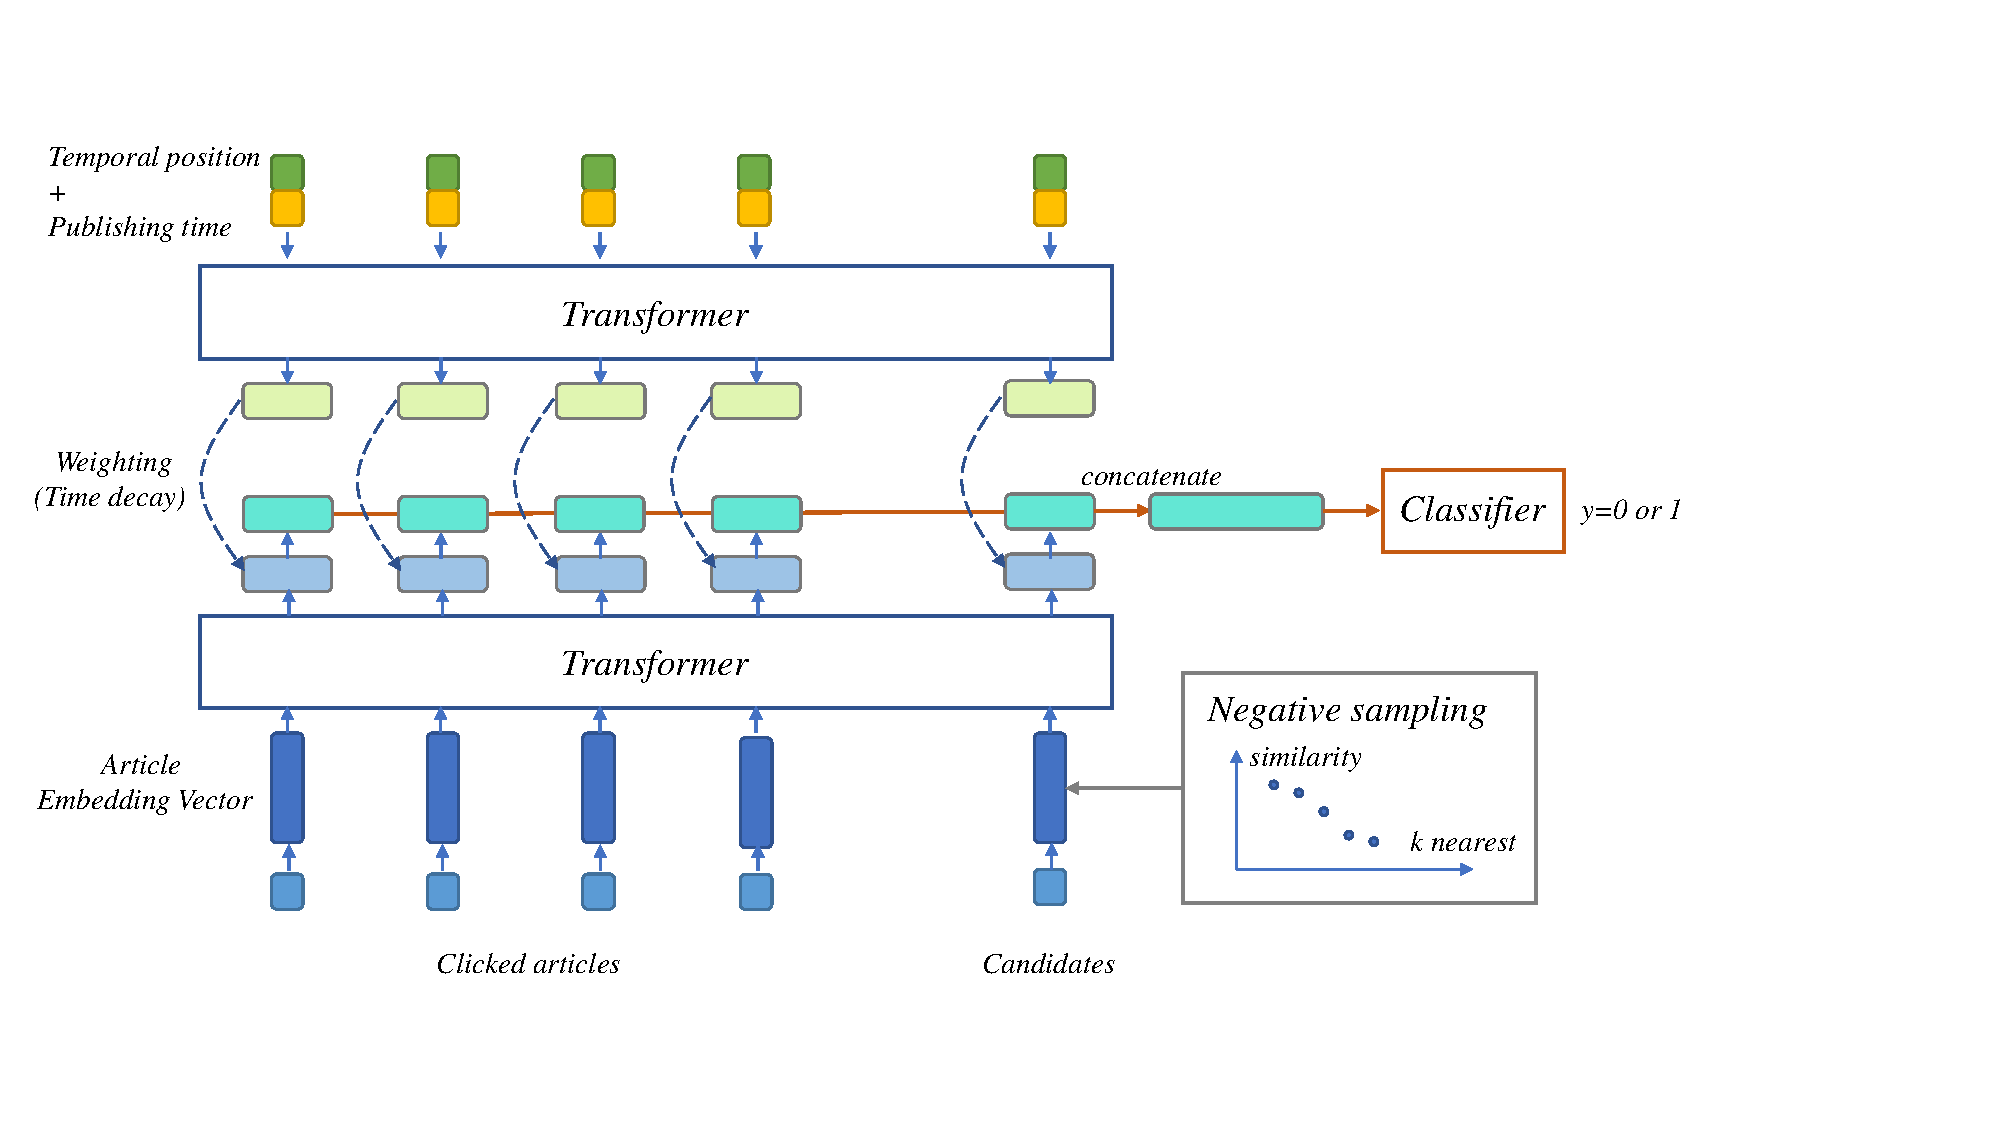
\includegraphics[width=12cm]{fig/architecture.pdf}
    \caption{An architecture of session-based news recommendation}
    \label{fig:architecture}
    % \Description[An architecture]{This is an architecture of session-based news recommendation}
\end{figure*}
\subsection{Article context embedding}
\label{sec:3.1}
To deal with the item-cold-start problem, it is necessary to consider the textual content of articles when recommending. For article textual content embedding, a common practice in Deep Natural Language Processing (NLP) is to use pre-training word embeddings, which use methods like Word2Vec and GloVe in a large text corpus of the target language. Using a classifer to model the profile of articles, we can capture the content similarity in the follow-up approaches.

Follwing the Article Content Embedding module in CHAMELEON~\cite{moreira_importance_2019}, we encode content information of the article through Convolution Neural Network (CNN) layers. With article content word embedding as input, we predict metadata attributes of an article, such as categories or tags. The last fully connected hidden layer can be regard as the high dimensional representation of article topic. 

\subsection{Sequential modeling with intra-session temporal weighting}
After Recurrent Neural Network (RNN) and Long Short-Term Memory (LSTM)~\cite{guo_streaming_2019,hidasi2015session,wang2019modeling} deployed in sequential prediction task, several recent work show the high capacity of self attention mechanism to model sequential information in recommendation scenario~\cite{kang_self-attentive_2018,liu2018stamp,xu2019time}.
\label{sec:3.2}
In machine translation field, to retrieve relevant words in the source language and to generate the next word in the target language, the Transformer model relies heavily on the proposed ``self-attention'' modules to capture complex structures in sentences. Inspired by this, we seek to build two transformer layers based upon the self-attention approach to model user behavior with ambiguity by leveraging intra-session time weightage. The whole architecture is depicted in \figref{fig:architecture}.
\subsubsection{Context encoder}
We transform the training sequence $\{(x_1,c_1,T_1),(x_2,c_2,T_2),...,(x_{T-1},c_{T-1},T_{T-1})\}$ into a fixed-length sequence with the maximum length $n$ in our model. If the session length is longer than $n$, we truncate it, leaving the latest $n$ interactions, and if the session length is shorter than $n$, we use zero padding to the left of the sequence. Then, we create an item embedding matrix $\mathbf{E}\in \mathbb{R}^{(I+1)\times D}$, where $D$ is the latent dimensionality, and $I$ is the number of items in training dataset, and the remaining $1$ dimension is used as the embedding for the padding item or items in testing dataset while not in training dataset. We retrieve $x_j$'s embedding vector through $\mathbf{E}$ as $E_{x_j}$ and concatenate it with context vector $c_j$, in order to represent items that are never seen during training. Then we feed the sequence of article embedding vectors into a multi-head attention transformer, trying to learn more complex interest of users. 

\subsubsection{Temporal encoder}
For temporal embedding, we encode publish time of a article and click time of a article. In order to extract periodic temporal change which is also known as seasonality, we not only encode the time of day but also the day of week into a one-hot vector. 

\subsubsection{Session representation}

\subsubsection{Model training}
Following some recommenders~\cite{wu_neural_2019,wu_neural_2019-1}, we use negative sampling techniques for model training. The goal of our training task is to maximize the similarity between the session representation vector $\mathbf{s}$
and the context vector of positive article (the last read article in session, denoted as $\mathbf{e_{+}}$), while minimizing the pairwise similarity between $\mathbf{s}$ and the negative samples $\mathbf{e_{-}}\in N$, where $N$ is the set of negative samples.  Similar to Bayesian Personalized Ranking~\cite{Rendle2009BPR}, we adopt method which compares the score of positive items and sampled negative items to compute pairwise ranking loss. The loss at a given session is defined as: 

\begin{equation}
    \begin{aligned}
    Loss(\theta) = - \frac{1}{|N|}\sum_{e_{-i}\in N} \left(log(\sigma(\mathbf{s} \mathbf{e_{+}^{T}})) 
    + log(\sigma(1-\mathbf{s} \mathbf{e_{-i}^{T}}))\right),
    \end{aligned}
\end{equation}

where $\sigma$ denotes the sigmoid function. We use the Adam optimizer to optimize loss function. 

\subsection{Negative sampling with inter-session temporal relation}
\label{sec:3.3}
The most straightforward and widely adopted negative sampling strategy is to randomly select samples from a non-interacted set of items or to follow popularity-biased sampling strategy, sampling from a global buffer with the last N clicks~\cite{moreira_news_2018}. Further, some consider the item frequency within interaction sequences as the weight of negative sampling process~\cite{li_learning_2018}, and some propose an adversarial training framework to adaptively generate negative examples~\cite{wang_neural_2018}, and others adopt efficient mini-batch learning algorithm to  integrate the whole negative samples~\cite{chen2020efficient}.

The major problem of randomly sampled items is that these items might be completely unrelated to the user, so it's too ``easy'' for the model
to learn and discriminate them from the target ones, leaving little contribution for the model optimization. On the contrary, a informative item should be able to confuse the model if it has or not discovered more complex hidden deep user interaction representations.

Highly inspired by Time-Aware Session-KNN~\cite{garg2019sequence} and Session-based CF Similarity~\cite{sottocornola2018session}, we compute session similarity between sessions $s_j$ and target session $s$ with time decay function, assigning lower weightage for sessions farther from $s$. Denote sessions $s_j$ and $s$ are represented as binary vectors $\vec{s_j}$ and $\vec{s}$ in the $n$-dimensional space of items (1 stands for corresponding items in the session, 0 otherwise). The cosine similarity is given by:

\begin{equation}
    sim(s, s_j) = \frac{<\vec{s_j}, \vec{s}>}{\sqrt{||\vec{s_j}|| \cdot ||\vec{s}||}},
\end{equation}

Then we use exponential function to smooth the temporal gap between sessions and the weight factor $w(s_j|s)$ represent the recency of session $s_j$ w.r.t $s$:
\begin{equation}
    w(s_j|s) = exp(-\frac{T(s)-T(s_j)}{\lambda}),
\end{equation}

where $\lambda$ is a hyperparameter to control the decay shape and  $\lambda>0, T(s) > T(s_j)$.

The neighborhood set $N(s)$ is then constructed by taking the top-K most
similar sessions using the similarity measure:
\begin{equation}
    sim_t(s, s_j) = sim(s, s_j) \cdot w(s_j|s),
\end{equation}

Then $N(s)$ is our strong candidates to confuse the model.